\documentclass[tikz,border=3pt]{standalone}
\usepackage{pgfplots}\pgfplotsset{compat=1.18}
\usetikzlibrary{arrows.meta,positioning,calc}
\begin{document}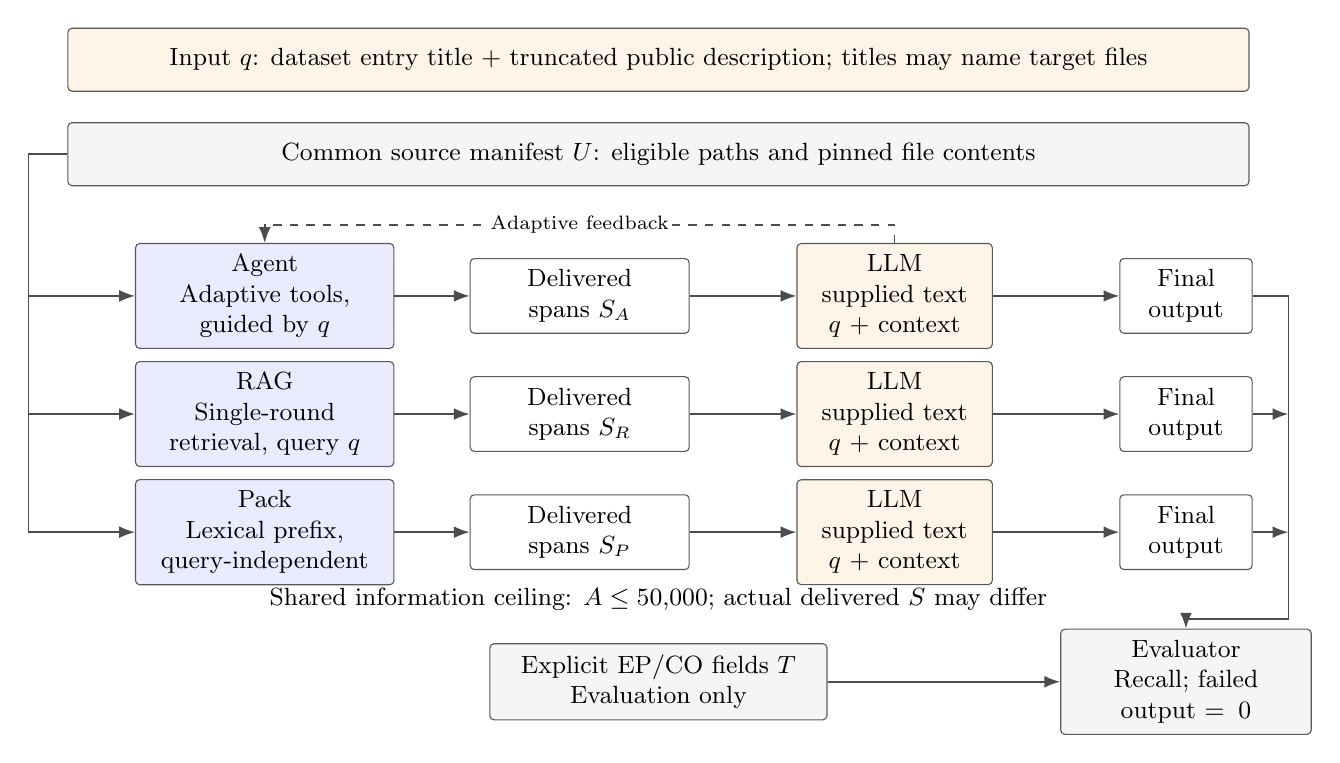
\begin{tikzpicture}

      \tikzset{box/.style={draw=black!65,rounded corners=1.5pt,align=center,
        minimum height=8mm,font=\small,inner sep=4pt},
        flow/.style={-{Latex[length=2mm]},draw=black!70,line width=.6pt}}
      \node[box,minimum width=15cm,fill=orange!9] at (7,5.5)
        {Input $q$: dataset entry title + truncated public description; titles may name target files};
      \node[box,minimum width=15cm,fill=gray!8] (u) at (7,4.3)
        {Common source manifest $U$: eligible paths and pinned file contents};
      \node[box,text width=3.0cm,fill=blue!8] (a) at (2,2.5)
        {Agent\\Adaptive tools, guided by $q$};
      \node[box,text width=3.0cm,fill=blue!8] (r) at (2,1.0)
        {RAG\\Single-round retrieval, query $q$};
      \node[box,text width=3.0cm,fill=blue!8] (p) at (2,-.5)
        {Pack\\Lexical prefix, query-independent};
      \node[box,text width=2.5cm] (sa) at (6,2.5) {Delivered spans $S_A$};
      \node[box,text width=2.5cm] (sr) at (6,1.0) {Delivered spans $S_R$};
      \node[box,text width=2.5cm] (sp) at (6,-.5) {Delivered spans $S_P$};
      \node[box,text width=2.2cm,fill=orange!9] (ma) at (10,2.5)
        {LLM\\supplied text $q$ + context};
      \node[box,text width=2.2cm,fill=orange!9] (mr) at (10,1.0)
        {LLM\\supplied text $q$ + context};
      \node[box,text width=2.2cm,fill=orange!9] (mp) at (10,-.5)
        {LLM\\supplied text $q$ + context};
      \node[box,text width=1.4cm] (pa) at (13.7,2.5) {Final\\output};
      \node[box,text width=1.4cm] (pr) at (13.7,1.0) {Final\\output};
      \node[box,text width=1.4cm] (pp) at (13.7,-.5) {Final\\output};
      \foreach \policy/\spans/\model/\pred in {a/sa/ma/pa,r/sr/mr/pr,p/sp/mp/pp} {
        \draw[flow] (u.west) -- (-1,4.3) |- (\policy.west);
        \draw[flow] (\policy) -- (\spans);
        \draw[flow] (\spans) -- (\model);
        \draw[flow] (\model) -- (\pred);
      }
      \draw[flow,dashed] (ma.north) -- (10,3.4) -- (2,3.4) -- (a.north);
      \node[font=\scriptsize,fill=white,inner sep=1pt] at (6,3.4) {Adaptive feedback};
      \node[font=\small,align=center] at (7,-1.35)
        {Shared information ceiling: $A\leq50{,}000$; actual delivered $S$ may differ};
      \node[box,text width=4.0cm,fill=gray!8] (t) at (7,-2.4)
        {Explicit EP/CO fields $T$\\Evaluation only};
      \node[box,text width=2.9cm,fill=gray!8] (eval) at (13.7,-2.4)
        {Evaluator\\Recall; failed output $=0$};
      \draw[flow] (t) -- (eval);
      \draw[flow] (pa.east) -- (15,2.5) -- (15,-1.6) -| (eval.north);
      \draw[flow] (pr.east) -- (15,1.0);
      \draw[flow] (pp.east) -- (15,-.5);
    
\end{tikzpicture}\end{document}
